\textit{This secion will go in depth with the extension-board created as an addon to the AQ M4 board. The extension-board was developed to act as a bridge between the PC and the CAN-bus using wireless communication.} \\

\subsubsection*{Wireless communication module}
An important part of the hardware is the wireless communication used between the PC and the drones.
The wireless communication module has severel requirements it needs to fulfill in order to make the whole system work as expected. A comparison table has been made in table \ref{tab:compare_table_wireless_communication} to find the wireless communication module that is best suited for the task. \\
The following wireless modules where considered and compared.
\begin{itemize}
	\item \textbf{ESP8266}
\end{itemize}

ESP8266 is a generel purpose 32 bit SOC with integrated WIFI 802.11 b/g/n support and buildin TCP/IP stack. It can be setup its own access point or it can connect to an existing wireless network.
It runs at 80MHz and can be flashed with a custom firmware. 
The SOC is sold as modules with different pinouts and features such as extra flash memory \footnote{\url{https://www.olimex.com/Products/IoT/MOD-WIFI-ESP8266/open-source-hardware}} and different antennas.
The chip has been on the marked for about two years and costs approximately 7\$. 
It has been widely used in DIY-projects due to its low price and because it requires a minimum of network knowledge to get up and running.\footnote{\url{http://www.esp8266.com/} - 43.000 posts in forum} When the SOC is shipped, it comes with a preloaded firmware which either accepts AT commands or LUA scripting depending on the version of the module. These simple programming interfaces makes it quick and easy to interface the cheap. \\
This leads to a large community where most of the problems have been found and solved already. Arduino has been ported to ESP8266 which makes it even easier to get it up and running. Their official Arduino GitHub has 2125 commits on their master branch at the time of writing\footnote{\url{https://github.com/esp8266/Arduino}} \\

\begin{itemize}
	\item \textbf{EMW3165}
\end{itemize}
EMW3165 is a SOC much like the ESP8266 supporting 802.11 b/g/n WIFI with buildin TCP/IP stack. As with ESP8266 it supports setting up an access point aswell as connecting to an existing network. It has a Cortex-M4 $\mu$C which run at 100MHz. 
It supports custom firmware and can be aswell be bought as different modules with different pinouts and antennas.
It differentiates itself from the ESP8266 by its higher frequency its 5 volts compatible pins \footnote{\url{https://hackadaycom.files.wordpress.com/2015/07/emw3165.pdf}} which makes it easier to connect other hardware which run 5 volt without the need of a logic level shifter. It has been on the marked for only one year and costs approximately 9\$. Since it is a newer board than ESP8266 it has not been used in the same number of applications and thereby has a smaller community behind\footnote{\url{http://www.emw3165.com/} - 200 posts in forum }. Their most active GitHub has 147 commits on their master branch at the time of writing\footnote{\url{https://github.com/SmartArduino/WiFiMCU}}.

\begin{itemize}
	\item \textbf{nRF51822}
\end{itemize}
nRF51822 is also a SOC, but it is using Bluetooth instead of WIFI. The nRF51822 $\mu$C is implementing BLE which is a power efficient way of sending and receiving data. The chip supports broadcasting which could be used in this project. The $\mu$C can be bought as a standalone component or mounted on modules as the two other $\mu$Cs. Different modules offers different types of antenna connectors or buildin antenna on the PCB. It has not been possible to find an Arduino ported firmware that supports this $\mu$C. To write a firmware for the $\mu$C it has to be done using Nordic Semiconductor's proprietary SDK. 


\begin{itemize}
	\item \textbf{XBee}
\end{itemize}
XBee is a module that implements the Zbee standard. The Xbee modules work as a wireless serial connection. The Xbee modules supports mesh networking which means the modules by themself figure out which module is closest and makes the connection. This idea makes sense in this application since there will be multiple drones and one computer. If one drone gets too far from the PC, it can just connect to one of the other drones closer to the PC.\\
The Xbee solution is ready to use and requires a minimum of programming to get up and running. The modules also support GPIO for digital in and output and analog input.

\begin{savenotes}
\begin{table}[H]
	\centering
	\begin{tabular}{@{}|l|l|l|l|l|l|l|l|@{}}
		\toprule
		\textbf{Product} & \textbf{Size} & \textbf{Weight} & \textbf{Price} & \textbf{Documentation} &  \textbf{Range}  & \textbf{Score} \\ \midrule
		ESP8266   &  24x16mm\footnote{\url{https://www.mikrocontroller.net/attachment/243558/fcc\_11.pdf} last visited 26 Maj} \hfill\{7\} & 1.5g\footnote{Measured by author on chemistry weight} \hfill\{8\} &   7.5\$\footnote{\url{http://www.seeedstudio.com/depot/ESP8266-based-WiFi-module-SPI-supported-p-2486.html} last visited 26 Maj}  \hfill\{9\}  &   Great community \hfill\{9\}  &    ?    &          33      		\\ \midrule
		EMW3165   &  32x16mm\footnote{\url{https://hackadaycom.files.wordpress.com/2015/07/emw3165.pdf} last visited 26 Maj} \hfill\{6\}  & 5g\footnote{\url{http://www.seeedstudio.com/depot/EMW3165-CortexM4-based-WiFi-SoC-Module-p-2488.html} last visited 26 Maj} \hfill\{2\} &  9\$\footnote{\url{http://www.seeedstudio.com/depot/EMW3165-CortexM4-based-WiFi-SoC-Module-p-2488.html}} \hfill\{8\}   &  Less available  \hfill\{3\}	        &    ?    &    19            		\\ \midrule
		nRF51822  &  18x10mm\footnote{\url{http://www.fanstel.com/Product/bluenor.html}last visited 26 Maj} \hfill\{8\}  & 3g\footnote{\url{http://www.seeedstudio.com/depot/MDBT40P\%C2\%A0\%C2\%A0nRF51822\%C2\%A0based\%C2\%A0BLE\%C2\%A0module-p-2503.html} last visited 26 Maj} \hfill\{4\}  &  7.5\$ \footnote{\url{http://www.seeedstudio.com/item_detail.html?p_id=2503} last visited 26 Maj} \hfill\{9\}   & Ok documented\hfill\{2\} 	        &   30 M\footnote{\url{https://dl.dropboxusercontent.com/u/54939426/Fanstel_BT600.pdf} last visited 26 Maj}  \hfill\{9\}     &               32 		\\ \midrule
		XBee      &  24.38x27.61mm \footnote{\url{http://www.digi.com/products/xbee-rf-solutions/modules/xbee-802-15-4\#specifications}} \{3\} & 3g \footnote{\url{http://www.digi.com/products/xbee-rf-solutions/modules/xbee-802-15-4\#specifications} last visited 26 Maj} \hfill\{4\} &   25\$\footnote{\url{https://www.sparkfun.com/products/11215} last visited 26 Maj}  \hfill\{4\}  &  Lots of DIY   \hfill\{9\}      &            91 M\footnote{\url{https://www.sparkfun.com/pages/xbee_guide}}  \hfill\{9\}  &             29       \\ \bottomrule
	\end{tabular}
	\caption{Comparisontable used to compare different wireless 		communication modules}
	\label{tab:compare_table_wireless_communication}
\end{table}
    \end{savenotes}

The products compared in \ref{tab:compare_table_wireless_communication} are chosen to have approximately same specs such as onboard antenna and no need for extra components.
The ESP8266 module based on the highest score but must of all because it is use in a wide range of applications and has a lot of activity on their official Arduino github. The weight of the module was measured after the decision was made. If it was heavier than the other modules it would still have been used due to the large number of projects using this module. In case help was needed to make the module work, plenty of projects is available online and they have an active forum\footnote{\url{http://www.esp8266.com/} last visited 26 Maj}

\subsubsection*{Microcontroller}
The list below shows the requirement for the microcontroller on the extension-board.
\begin{itemize}
	\item \textbf{CAN-controller} to communicate with the AQ M4 board.
	\item \textbf{2 UART} to communicate with the ESP8266-module and with a PC for debugging purpose.
	\item \textbf{Small package} such as QFN64 (9*9mm)
\end{itemize}

The AT90CAN128 was chosen since the author and SDU had experience programming and using that microcontroller. It meets the requirements as well since it has built-in CAN controller,  two UARTS and is available in QFN64 package.
Kjeld Jensen has been in front of the development of the Frobomind-controller\footnote{\url{http://www.frobomind.org/index.php/FMCtrl:FroboMind\_Controller} last visited 22 Maj}, which uses the AT90CAN128 microcontroller.
Since the Frobomind-controller was available the author could start developing the firmware while the PCB for the ladybirds were made.

\subsubsection*{Block Schematic}
The block schematic shown in figure \ref{fig:PCB_block} was created by the author. It was then given to Carsten Albertsen who created the schematic and did rest of the creation of the PCB. Some time was spend  debugging since there was an error in the ISP pins. Later on the author had to make a correction to the board since a pin(GPIO15) on the ESP8266 that had to be grounded in order to select booting from the flash.
\begin{figure}[H]
    \center
    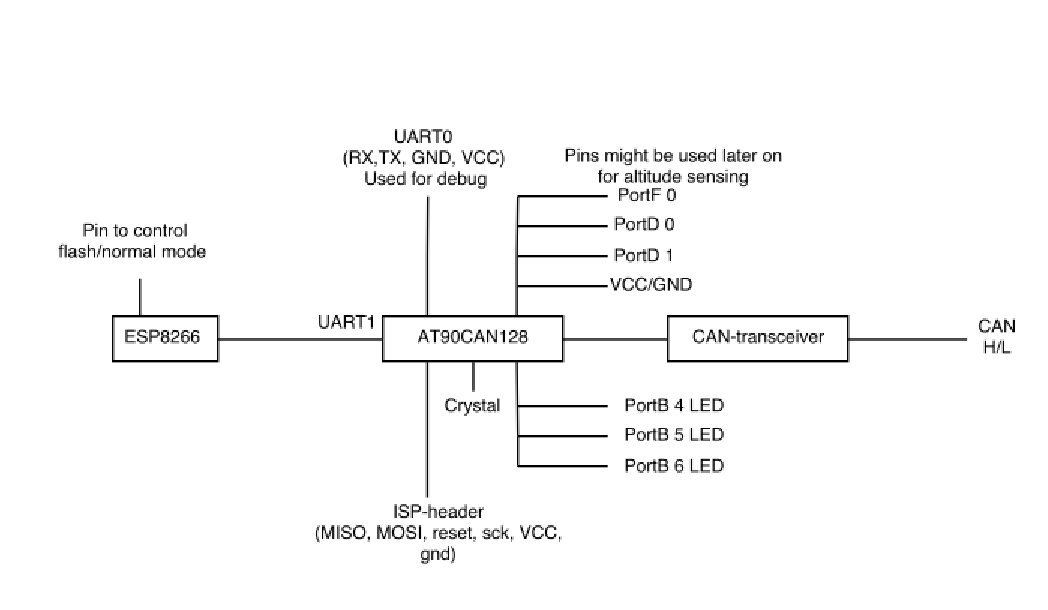
\includegraphics[width=0.9\textwidth]{graphics/PCB_block_v3.eps}
    \caption{Block schematic of the extension-board developed to AQ M4. It can be seen that the ESP8266 chip is connected to the At90CAN128 using UART1 and that the AtMega is connect to a can-transceiver which  communicates with the AQ M4 board.}
    \label{fig:PCB_block}
\end{figure}

\subsubsection*{Pins}
A few pins where made available through solder pads for easy access if needed later on.

The following pins where available as solder pads:
\begin{itemize}
	\item PortF 0 - Alternative function as ADC, channel 0
	\item PortD 0 - Alternative function as interrupt, INT0 and I2C, SCL
	\item PortD 1 - Alternative function as interrupt, INT1 and I2C, SDA
\end{itemize}
In case the onboard baromter is not accurate enough, an alternative distance could be used to measure the drones altitude with respect to the ground.
PortF0 has been made available since some distance sensors give output as an analogue value. 
An example of such sensor is an Infrared proximity sensor.\footnote{\url{http://www.sharpsma.com/webfm\_send/1208}} \\
As an alternative type of distance sensor, a ultrasoinc could be used such as HCSR04.
As output it gives a binary output with high-time proportional with the distance.\footnote{\url{http://www.micropik.com/PDF/HCSR04.pdf}}.
To detect the high-time, one of PortD1/0 would be useful. \\

Which type of sensor suits best as a distance sensor to provice altitude information to the drone is ouf of the scope of this report. The PCB has just been made ready to different types of sensors.

\subsubsection*{Debug/ISP}
In the final schematic UART0 and ISP pins where combined in one pinheader for easy access through one cable. \Mathias{Refer to image of board}
To program the AtMega the ISP pins where required to be easy accessable. 
UART0 was made accessable to be used as debug and programming of the ESP8266 board.
The idea was to setup the AtMega as UART passthrough from UART0 to UART1.
Due to a mistake\footnote{The wrong pair of MISO/MOSI pins where made available in the ISP-header. The correct pair of MISO/MOSI is also RXD0/TXD0 as alternative function} in the final schematic, both UART0 and UART1 where made accessable trough the ISP/debug header. 
This ended up making it easier to program the ESP8266-board without using the AtMega as UART passthrough.



\begin{figure}[H]
    \centering
    \begin{subfigure}[b]{0.45\textwidth}
        \includegraphics[width=\textwidth]{graphics/extension_board_up}
        \caption{Top-view of the developed extension-board. If looking carefully, the ISP-fix can be seen between the ESP-8266 module and the Debug/ISP pins.}
        \label{fig:tiger}
    \end{subfigure}
    ~ %add desired spacing between images, e. g. ~, \quad, \qquad, \hfill etc. 
    %(or a blank line to force the subfigure onto a new line)
    \begin{subfigure}[b]{0.51\textwidth}
        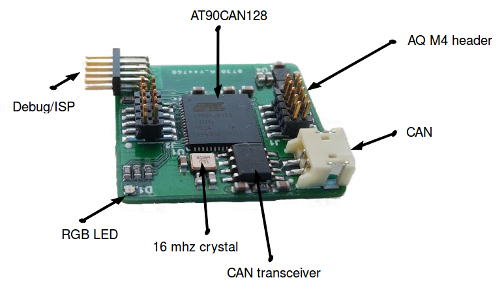
\includegraphics[width=\textwidth]{graphics/extension_board_down}
        \caption{Bottom-view of the developed-extension board. The two connects for the AQ M4 board can be seen pointing up. The CAN-connect is of same type mounted on the AQ M4 board.}
        \label{fig:mouse}
    \end{subfigure}
    \caption{Top and bottom view of the extension-board}\label{fig:extension_board}
\end{figure}



\subsubsection*{Test of WIFI range}
A test of the wifi was conducted in order to test the range of the ESP8266 module. Test of the AtMega is done in section \ref{sec:extensionboard_firmware}

To make the test, the fimrware of the ESP8266 module had to be flashed to specify which access point it should connect to. How the networking was configured can be seen in section \ref{sec:server_configuration}.

The first test was conducted by pinging the module from the authors laptop 200 times, 10 hz with a packet size of the dataframe used in the application.\footnote{See more about the size and content in section \ref{sec:shizzle}}. The purpose of the test was to see how the latency behaves when the distance is increased and when it stops receiving or transmitting packets.

Figure \ref{fig:wifi_ping_test} shows the results.

\begin{figure}[H]
    \center
    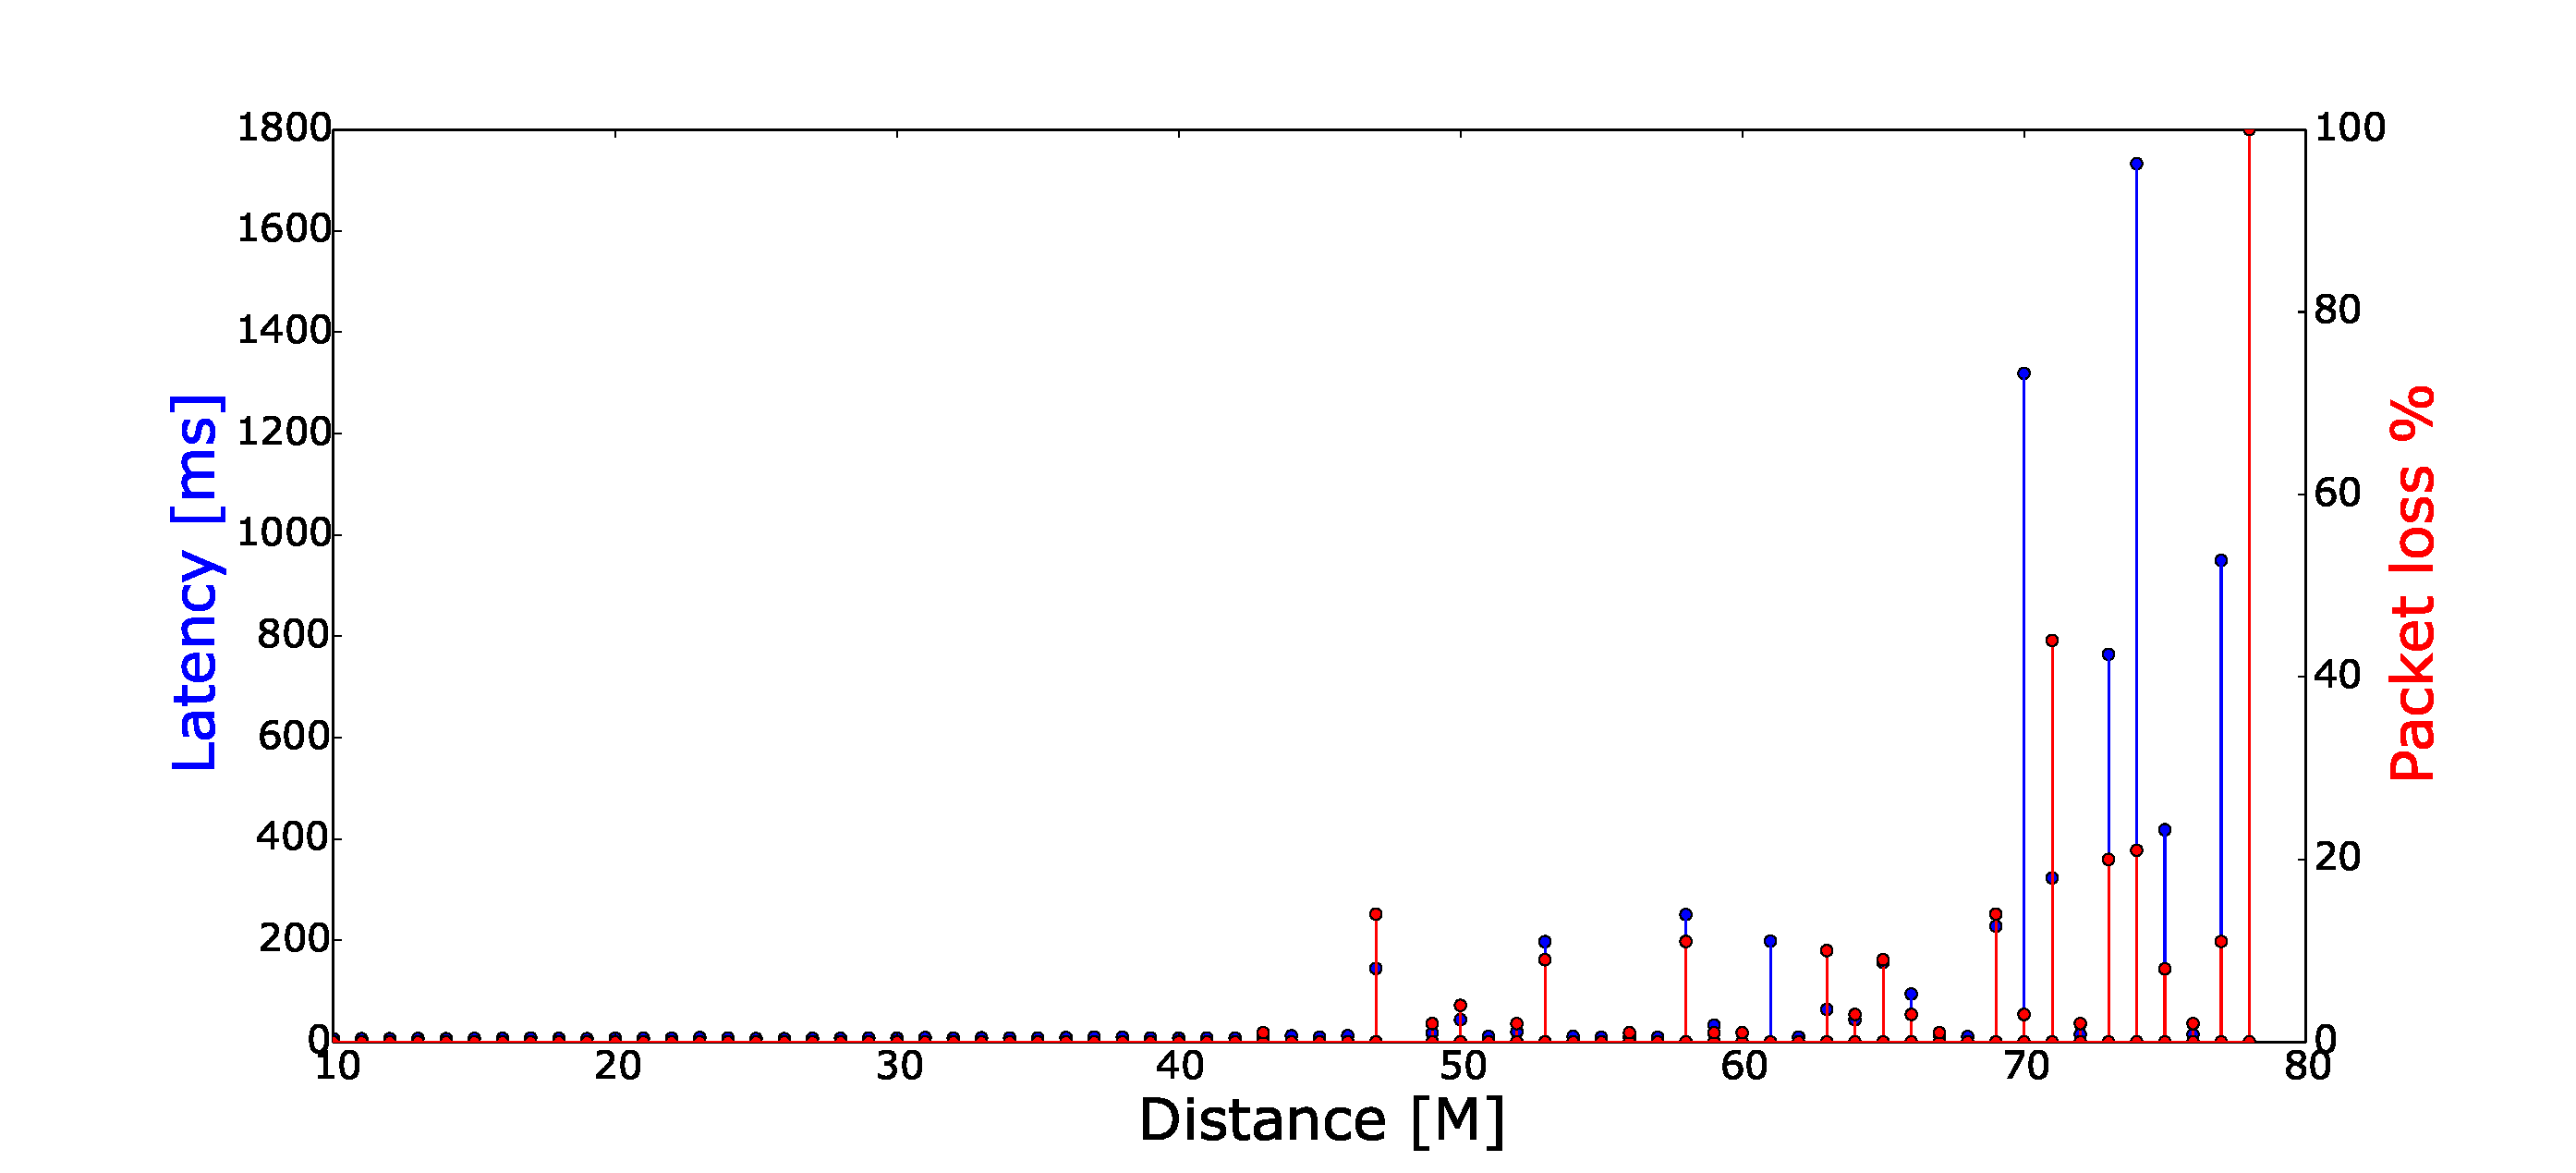
\includegraphics[width=0.85\textwidth]{graphics/wifi_test_latency_1.eps}
  \caption{Tasks diagram showing overview of the running tasks on the At90Can128}
    \label{fig:wifi_pingtest}
\end{figure}

Another test was done where the authors laptops sends datapackages to the ESP8266 module. The rests shows for how long a distance the module can be from the laptop and still receive valid packets. CRC-16 was used to validate the content of the packets. \footnote{See more about this in section \ref{sec: extensionboard_software}}

\begin{figure}[H]
    \center
    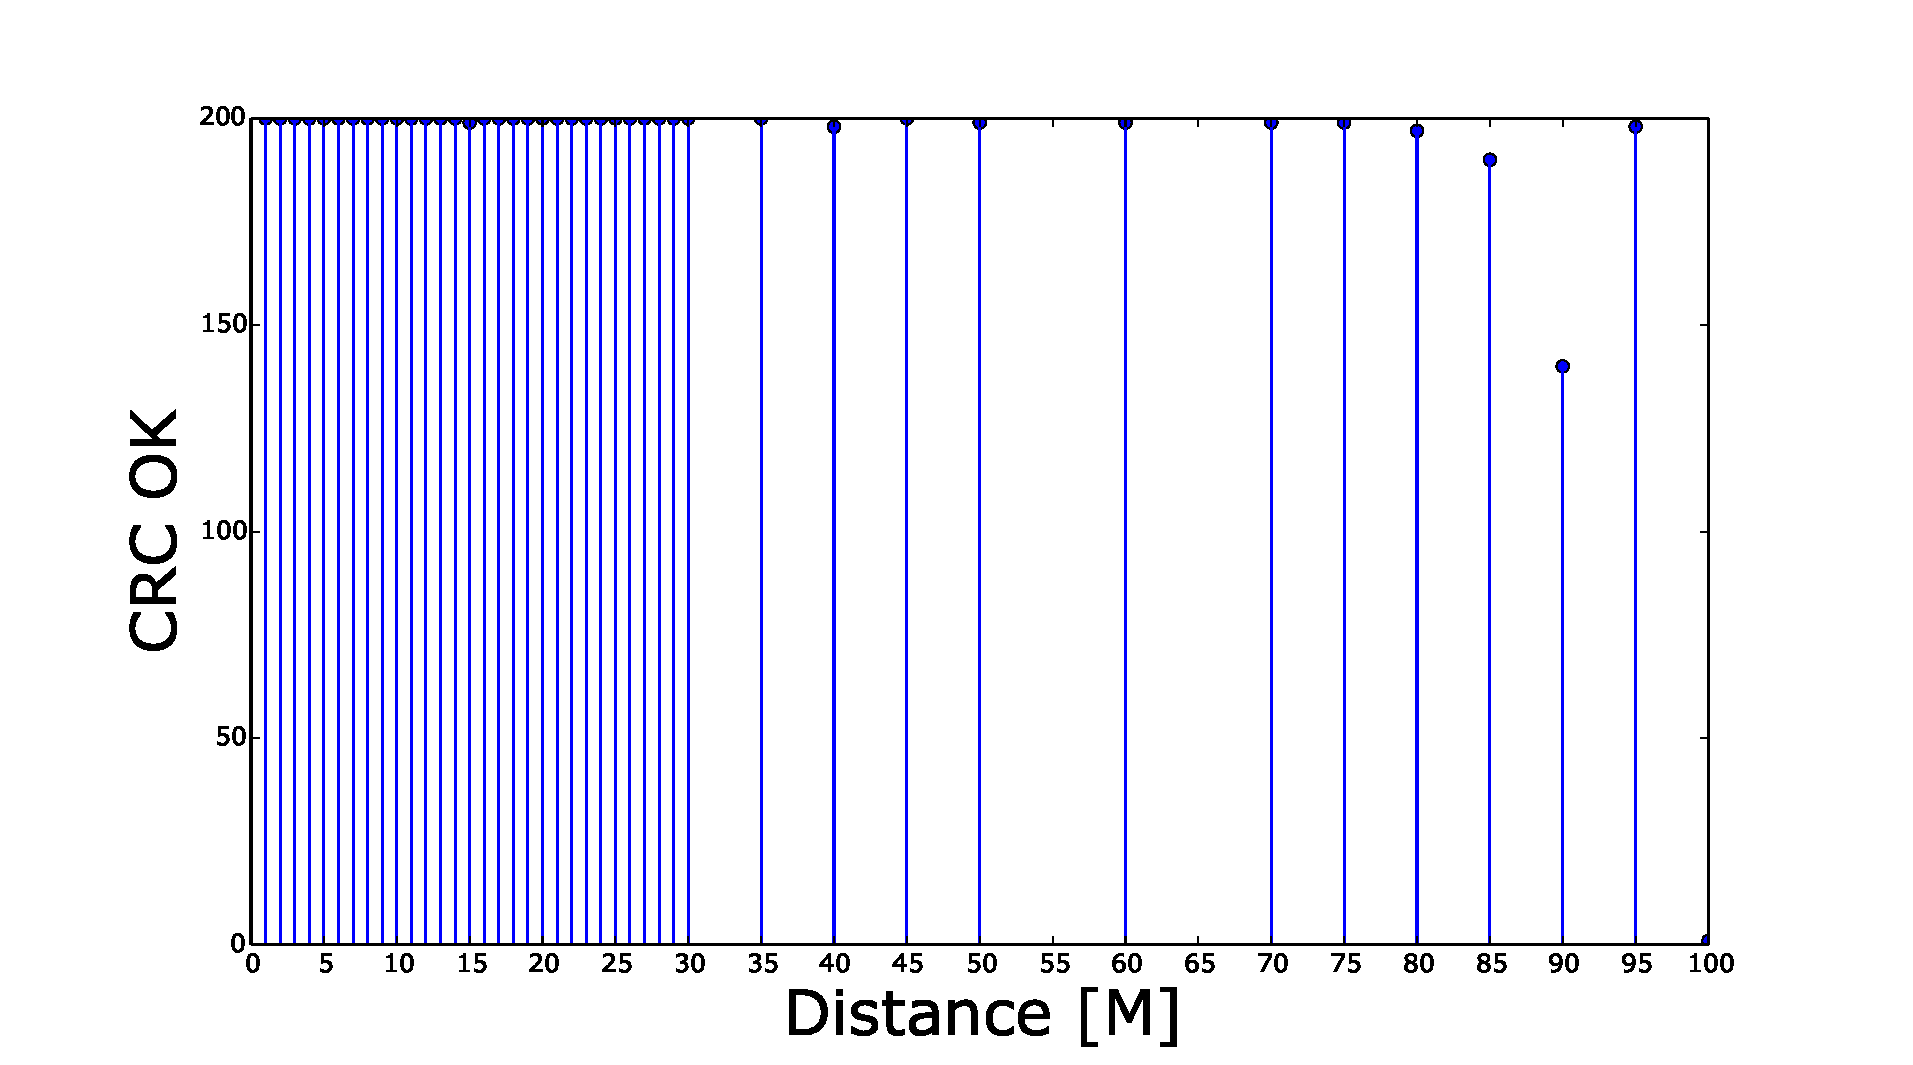
\includegraphics[width=0.85\textwidth]{graphics/crc_distance_check.eps}
	\caption{Two modules were connected to one laptop which transmitted datapackets to both modules. Another laptop was connected to one extension-board at a time to check it received all of its packets without error}
    \label{fig:wifi_pingtest}
\end{figure}


A final test was made to see how the modules behave when two modules are receiving the packets. At 10 hz datapackets was sent to two modules at a distance of 10 meters.
\begin{figure}[H]
    \centering
        \includegraphics[width=0.5\textwidth]{graphics/laptop_extenbioard_crc_check}
        \caption{}
        \label{fig:tiger}
\end{figure}
Both modules received their packets without CRC error.

It can be concluded that the chosen wifi modules, ESP8266 works well. At a distance of 100 meters it drops.... and that .. and it indicates that the communication works when more than one ESP8266 is connected to the laptop using WIFI.


